\documentclass[11pt,a4paper]{article}\usepackage[T1]{fontenc}\usepackage[utf8]{inputenc}\usepackage{lmodern,geometry,hyperref,tikz}\geometry{margin=21mm}\setlength{\parindent}{0pt}\setlength{\parskip}{5pt}\setlength{\emergencystretch}{3em}\begin{document}
\section*{Generált cellaszimuláció és követelménybizonyíték}
Létrehozva: 2026-10-15 16:28 +02:00. ETA: 60--90 perc; deklarált csomag és tesztek, rövid fizikai futások, mérési összekötés, animáció/PDF.
\paragraph{Cél.} A meglévő logikai követelménypéldát konkrét, generált robotmodellhez és natív MuJoCo-futáshoz kötni. A forrás a meglévő egyszerűsített FANUC-modellt importálja; egy kis fix vákuumcsésze és a forgatókönyv adatai új deklarációk. Nincs RL vagy tanítás. A megfogás ideális weld-kényszer: nem súrlódásos ujj-, tömítés- vagy valódi biztonsági igazolás.
\paragraph{Tulajdonosok.} Core fordítás, identitás és checked értékfrissítés. Query referencia- és mezőfeloldás. Geometry/FK és Formats/MJCF a robotot olvassa/írja. Formats traceability modul: típussal és referenciával kötött mérési szabályok, csomag és eredménybefogadás. Simulator: meglévő RobotRun, JointMotion/MissionMotion, MuJoCoSceneAdapter; az új kliens csak jelenetet komponál, végrehajt és megfigyel. MuJoCo végzi az időléptetést és kényszermegoldást. Kawamirai és az RL érintetlen.
\paragraph{Állapot.} Transformation fe7d6436e77d, helyi korábbi emitter/trace javításokkal; upstreammel egyezik. Simulator 2538cf9dba27, dirty meglévő checkout, a friss upstreamhez képest 62 commit hátrány. Nincs tiszta/üres szinkronizálható checkout; a meglévő Python-felületet használjuk, a többi módosítás megőrzendő. Nem állítunk tiszta klónos hordozhatóságot és nem váltunk ágat/worktree-t. A két tulajdonos között fájl-artifact a határ, nincs új Cargo-függőség vagy sibling override.
\paragraph{Érintett fájlok.} Formats traceability.rs és traceability/simulation.rs; examples/trace\_simulation.rs; tests/trace\_simulation.rs; data/paper/meta\_simulation\_case.hymeko és traceability\_simulation.hymeko; célzott README és szimbólumindex. Simulator python/requirement\_simulation.py és python/tests/test\_requirement\_simulation.py. A meglévő RobotRun, MissionMotion és scene adapter nem másolódik. A teljes kezdeti mentés a dátumos reports alatt. CORE.YAML=[]; nincs projektfüggőség-változás.
\paragraph{Szerződés és bizonyíték.} A forrásnézetekben a hat mérési eredmény előbb Unknown; a korábbi szintetikus pass értékek nem léphetnek át észrevétlenül. Előáll: robot-MJCF, deklarált pálya és szabályok, referenciák, kezdeti SysML/DOT/CSV. A futás naplózza a fizikai időt, pozíciókat, sebességeket, kontaktusokat, attachment állapotot. Utána a Core támogatott leaf update-jével visszaírt eredményekből ismét három nézet készül. Eltérő modell-digest, hiányzó/NaN mérés és nem támogatott szabály nem lehet sikeres eredmény.
\paragraph{Protokoll.} Maximum 10 s fizikai idő futásonként, 1 ms lépés, legfeljebb 5 futás: baseline három determinisztikus ismétlése, külön megállási próba, külön nyitott megfogó hibakontroll. Előre rögzített limitek: állomási TCP-hiba 0.5 mm; ciklus 4 s; ismétlés 0.1 mm; megállás 200 ms, legalább 50 ms folyamatosan alacsony sebesség mellett. A további megfogási/diagnosztikai invariánsok a deklarált source-szabályokban. A fizikai modell vagy szabályozó paramétereinek változtatását külön futás és új receipt jelöli. Sikertelen követelmény megmarad eredménynek; a küszöböt nem lazítjuk a PASS érdekében.
\paragraph{V\&V és korlát.} Előbb forrás/projekció/negatív szabálytesztek; utána natív beolvasás, FK és world-összeállítás; csak ezek után rövid fizikai futás. A szabályok határértéke, stale digest, hiányzó eredmény és nyitott gripper hibája tesztelendő. A pozíciópontosság és repeatability a deklarált állomási protokollra vonatkozik; a teljes pályahiba külön érték. Az ideális vákuum eredménye feltételes modellszimuláció, nem gyártói vagy hardveres verifikáció.
\paragraph{Erőforrás, visszaállítás, lezárás.} Legfeljebb 4 build-job, 50\,000 fizikai lépés kezdeti keret, 16 GB alatt tervezett memória, legfeljebb 200 képkocka. Nincs throughput-benchmark, profilozás vagy hard-real-time állítás. Haladás futásonként és legfeljebb másodpercnyi szimulált időnként. Csak új futáskönyvtárakba írunk. Nincs commit/push/merge/stash/reset. Kimenet: MJCF, mérési JSON/CSV, jelenetnyom, PNG/GIF, PDF és checksumok; Samba-másolat byte-ellenőrzéssel.
\paragraph{Mért eltérés és célzott kiegészítés.} Az 1 ms-os első kampány után a megállási próba nem kvalifikált: a csukló utolsó mintabeli sebessége 0.418 rad/s volt, miközben a ritkább pozícióminták nettó változása közel nulla. A sűrűbb megfigyelés újrafutása byte-azonos pozíciósort adott, tehát a naplózás nem változtatta meg a pályát. Egyetlen változós lépésfinomítás: 0.5 ms, azonos fizikai modell, szabályozógain és követelményküszöb. Először külön stop-próba, utána a végleges öt eset. A célzott diagnosztikákkal a keret legfeljebb 75\,000 lépés; a 16 GB korlát marad. A régi hibás eredmény és forrás megmarad. A RobotRun fixed-base ellenőrzése név szerint deklarált, gyökérszintű passzív munkadarabokra bővült, a nem deklarált szabad testek elutasítása tesztelt. Cenzorált mérésnél alsó/felső korlát dönt a bizonyított hibáról vagy ismeretlenről; hiányzó adatra nincs kitalált mérési érték.
\begin{center}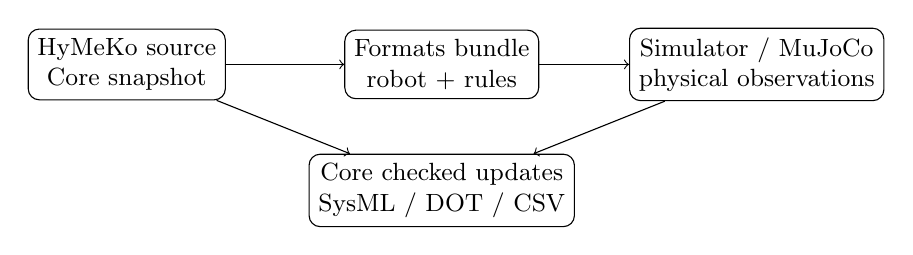
\begin{tikzpicture}[every node/.style={draw,rounded corners,align=center,font=\small}]\node (s) at (0,0) {HyMeKo source\\Core snapshot};\node (b) at (4,0) {Formats bundle\\robot + rules};\node (m) at (8,0) {Simulator / MuJoCo\\physical observations};\node (r) at (4,-1.6) {Core checked updates\\SysML / DOT / CSV};\draw[->] (s)--(b);\draw[->] (b)--(m);\draw[->] (m)--(r);\draw[->] (s)--(r);\end{tikzpicture}\end{center}\end{document}